% Options for packages loaded elsewhere
\PassOptionsToPackage{unicode}{hyperref}
\PassOptionsToPackage{hyphens}{url}
%
\documentclass[
]{article}
\title{BODY FAT}
\author{John Karuitha}
\date{Sunday, August 01, 2021}

\usepackage{amsmath,amssymb}
\usepackage{lmodern}
\usepackage{iftex}
\ifPDFTeX
  \usepackage[T1]{fontenc}
  \usepackage[utf8]{inputenc}
  \usepackage{textcomp} % provide euro and other symbols
\else % if luatex or xetex
  \usepackage{unicode-math}
  \defaultfontfeatures{Scale=MatchLowercase}
  \defaultfontfeatures[\rmfamily]{Ligatures=TeX,Scale=1}
  \setmainfont[]{firacode}
\fi
% Use upquote if available, for straight quotes in verbatim environments
\IfFileExists{upquote.sty}{\usepackage{upquote}}{}
\IfFileExists{microtype.sty}{% use microtype if available
  \usepackage[]{microtype}
  \UseMicrotypeSet[protrusion]{basicmath} % disable protrusion for tt fonts
}{}
\makeatletter
\@ifundefined{KOMAClassName}{% if non-KOMA class
  \IfFileExists{parskip.sty}{%
    \usepackage{parskip}
  }{% else
    \setlength{\parindent}{0pt}
    \setlength{\parskip}{6pt plus 2pt minus 1pt}}
}{% if KOMA class
  \KOMAoptions{parskip=half}}
\makeatother
\usepackage{xcolor}
\IfFileExists{xurl.sty}{\usepackage{xurl}}{} % add URL line breaks if available
\IfFileExists{bookmark.sty}{\usepackage{bookmark}}{\usepackage{hyperref}}
\hypersetup{
  pdftitle={BODY FAT},
  pdfauthor={John Karuitha},
  hidelinks,
  pdfcreator={LaTeX via pandoc}}
\urlstyle{same} % disable monospaced font for URLs
\usepackage[margin=1in]{geometry}
\usepackage{graphicx}
\makeatletter
\def\maxwidth{\ifdim\Gin@nat@width>\linewidth\linewidth\else\Gin@nat@width\fi}
\def\maxheight{\ifdim\Gin@nat@height>\textheight\textheight\else\Gin@nat@height\fi}
\makeatother
% Scale images if necessary, so that they will not overflow the page
% margins by default, and it is still possible to overwrite the defaults
% using explicit options in \includegraphics[width, height, ...]{}
\setkeys{Gin}{width=\maxwidth,height=\maxheight,keepaspectratio}
% Set default figure placement to htbp
\makeatletter
\def\fps@figure{htbp}
\makeatother
\setlength{\emergencystretch}{3em} % prevent overfull lines
\providecommand{\tightlist}{%
  \setlength{\itemsep}{0pt}\setlength{\parskip}{0pt}}
\setcounter{secnumdepth}{-\maxdimen} % remove section numbering
\newlength{\cslhangindent}
\setlength{\cslhangindent}{1.5em}
\newlength{\csllabelwidth}
\setlength{\csllabelwidth}{3em}
\newlength{\cslentryspacingunit} % times entry-spacing
\setlength{\cslentryspacingunit}{\parskip}
\newenvironment{CSLReferences}[2] % #1 hanging-ident, #2 entry spacing
 {% don't indent paragraphs
  \setlength{\parindent}{0pt}
  % turn on hanging indent if param 1 is 1
  \ifodd #1
  \let\oldpar\par
  \def\par{\hangindent=\cslhangindent\oldpar}
  \fi
  % set entry spacing
  \setlength{\parskip}{#2\cslentryspacingunit}
 }%
 {}
\usepackage{calc}
\newcommand{\CSLBlock}[1]{#1\hfill\break}
\newcommand{\CSLLeftMargin}[1]{\parbox[t]{\csllabelwidth}{#1}}
\newcommand{\CSLRightInline}[1]{\parbox[t]{\linewidth - \csllabelwidth}{#1}\break}
\newcommand{\CSLIndent}[1]{\hspace{\cslhangindent}#1}
\usepackage{pdflscape}
\newcommand{\blandscape}{\begin{landscape}}
\newcommand{\elandscape}{\end{landscape}}
\usepackage[default]{sourcesanspro}
\usepackage[T1]{fontenc}
\usepackage{amsmath}
\usepackage{subcaption}
\usepackage{booktabs}
\usepackage{longtable}
\usepackage{array}
\usepackage{multirow}
\usepackage{wrapfig}
\usepackage{float}
\usepackage{colortbl}
\usepackage{pdflscape}
\usepackage{tabu}
\usepackage{threeparttable}
\usepackage{threeparttablex}
\usepackage[normalem]{ulem}
\usepackage{makecell}
\usepackage{xcolor}
\ifLuaTeX
  \usepackage{selnolig}  % disable illegal ligatures
\fi

\begin{document}
\maketitle

{
\setcounter{tocdepth}{2}
\tableofcontents
}
\hypertarget{introduction}{%
\section{\texorpdfstring{\textbf{1
Introduction}}{1 Introduction}}\label{introduction}}

The dataset \texttt{Bodyfat4} shows the body fat percentage for 252
individuals. There are 13 variables. First, there is an identifier
variable (IDNO) that uniquely identifies each observation. The body fat
(BODYFAT) content is the dependent variable. The remaining eleven (11)
are the independent variables that could explain the variability of body
fat among the different individuals. The dataset has no missing values.
The task is to build a regression model that can be useful in explaining
and predicting the body fat of individuals. The data analysis proceeds
as follows. In the next section, I visualize the data and then present
summary statistics. Next, I present the correlation analysis and then
the results of the regression.

\hypertarget{analysis-and-interpretation-of-results}{%
\section{\texorpdfstring{\textbf{2 Analysis and Interpretation of
Results}}{2 Analysis and Interpretation of Results}}\label{analysis-and-interpretation-of-results}}

In this section, we describe the data by generating summary statistics
and a correlation matrix. We then visualize the data.

\hypertarget{descriptive-statistics}{%
\subsection{\texorpdfstring{\textbf{2.1 Descriptive
Statistics}}{2.1 Descriptive Statistics}}\label{descriptive-statistics}}

Table () below shows a summary of the variables. Among the dependent
variables, the highest variability(SD- standard deviation) is observed
between individuals' abdomen, age, and weight. For the dependent
variable body fat, the mean is 18.9, with an unusual observation of zero
body fat as the minimum value. Given that there is a base level of body
fat necessary for humans to survive, this is a peculiar observation. For
robustness, it would be advisable to drop this case.

\begin{table}

\caption{\label{tab:unnamed-chunk-2}Summary Statistics}
\centering
\fontsize{12}{14}\selectfont
\begin{tabular}[t]{lrrrrrrrr}
\toprule
Variable & Complete & Mean & SD & Min & Q1 & Median & Q3 & Max\\
\midrule
bodyfat & 1 & 18.939 & 7.7509 & 0.000 & 12.800 & 19.000 & 24.60 & 45.100\\
density & 1 & 1.056 & 0.0190 & 0.995 & 1.041 & 1.055 & 1.07 & 1.109\\
age & 1 & 44.885 & 12.6020 & 22.000 & 35.750 & 43.000 & 54.00 & 81.000\\
weight & 1 & 178.924 & 29.3892 & 118.500 & 159.000 & 176.500 & 197.00 & 363.150\\
height & 1 & 70.149 & 3.6629 & 29.500 & 68.250 & 70.000 & 72.25 & 77.750\\
\addlinespace
adiposity & 1 & 25.437 & 3.6481 & 18.100 & 23.100 & 25.050 & 27.32 & 48.900\\
thigh & 1 & 59.406 & 5.2500 & 47.200 & 56.000 & 59.000 & 62.35 & 87.300\\
abdomen & 1 & 92.556 & 10.7831 & 69.400 & 84.575 & 90.950 & 99.33 & 148.100\\
ankle & 1 & 23.102 & 1.6949 & 19.100 & 22.000 & 22.800 & 24.00 & 33.900\\
hip & 1 & 99.905 & 7.1641 & 85.000 & 95.500 & 99.300 & 103.53 & 147.700\\
\addlinespace
wrist & 1 & 18.230 & 0.9336 & 15.800 & 17.600 & 18.300 & 18.80 & 21.400\\
knee & 1 & 38.590 & 2.4118 & 33.000 & 36.975 & 38.500 & 39.92 & 49.100\\
\bottomrule
\multicolumn{9}{l}{\rule{0pt}{1em}Source: Author's construction from title}\\
\end{tabular}
\end{table}

\hypertarget{correlation-analysis}{%
\subsection{\texorpdfstring{\textbf{2.2 Correlation
Analysis}}{2.2 Correlation Analysis}}\label{correlation-analysis}}

In this section, I present the pairwise plots for all the variables,
excluding the identifier variable (IDNO). The upper part of the figure
shows the pairwise correlation between the variables. The main diagonal
shows the distribution of the respective variable. For instance, the
plot on the intersection of the first row and the first column shows the
distribution of the body fat (BODYFAT) variable. The lower half shows
the scatter plots for each pair of variables.

\begin{landscape}

Figure 3.1:

\includegraphics{karuitha_wits_bmi_files/figure-latex/unnamed-chunk-3-1.pdf}

\end{landscape}

Figure () below is an extension of Figure () above and visualizes the
correlation between the variables with the circle sizes showing the size
of the correlation while the colour shows the direction (positive or
negative).The red colouring corresponds to negative correlation while
blue shows positive correlation. White is neutral indicating little
correlation in either direction. It is important to note that in
interpreting this visualization, I am Ignoring the main diagonal (which
is the correlation of a variable with itself).

\includegraphics{karuitha_wits_bmi_files/figure-latex/unnamed-chunk-4-1.pdf}

The correlation shows the high levels of correlation between most of the
variables in the dataset. I focus on the dependent variables as a high
degree of correlation between them leads to the problem of
multicollinearity. Using a cut off of 0.7 that some researchers have
used (). The correlation analysis shows 18 pairs of independent
variables have a correlation beyond the threshold of 0.7. In the cases
where correlation exceeds the threshold, the variables involved are
Adiposity, weight, and abdomen (6 times each), knee, thigh and hip (5
times each), density (twice), and wrist (once). when we lower the
threshold to 0.6, we get 25 pairs of variables with correlation between
the threshold.

Multicollinearity is a problem because the independent variables in a
regression model should ideally be independent. If not, the regression
coefficient estimates become unstable (that is they vary a lot). The
reduced precision of the estimates reduces the predictive power of the
model (Frost 2019a). Scholars have suggested several solutions to the
multicollinearity problem. The first is to drop the variables that
exhibit multicollinearity. The second common technique is to use
principal component analysis (PCA) to generate a new set of new
variables (called components) that are linear combinations of the
original variables but that have low correlation between them. In the
next section, I describe and run the principal components analysis.

\hypertarget{principal-components-analysis-pca}{%
\subsection{\texorpdfstring{\textbf{2.3 Principal Components Analysis
(PCA)}}{2.3 Principal Components Analysis (PCA)}}\label{principal-components-analysis-pca}}

Principal components analysis (PCA) is a technique for dimension
reduction, increasing interpretability while minimizing the loss of
information (Jolliffe and Cadima 2016). PCA is especially useful where
there are many variables in a dataset or as in this case where variables
are highly correlated. The dimensions of the body fat dataset could be
reduced to get rid of the highly correlated dependent variables by
creating a new set of fewer variables called principle components that
are not correlated. The principal components are linear combinations of
the original variables that capture much of the variation in the
original dataset. In this section, I construct principal components and
discuss the applicability and limitations of the PCA analysis.

\hypertarget{running-pca}{%
\subsubsection{\texorpdfstring{\textbf{2.3.1 Running
PCA}}{2.3.1 Running PCA}}\label{running-pca}}

PCA is sensitive to differences in scale between the variables used.
Hence, it is recommended to first scale the variables (Zhu, Ge, and Song
2017). In this case, I scale the variables by subtracting the mean and
dividing by the standard deviation.

\begin{verbatim}
## $sdev
##  [1] 2.5770 1.2467 1.0196 0.7857 0.6513 0.5231 0.4406 0.3389 0.2628 0.2058
## [11] 0.1729
\end{verbatim}

\begin{table}
\caption{\label{tab:unnamed-chunk-5}Principal Components}
\begin{table}

\centering
\fontsize{12}{14}\selectfont
\begin{tabular}[t]{lrrrrrrrrrrr}
\toprule
  & PC1 & PC2 & PC3 & PC4 & PC5 & PC6 & PC7 & PC8 & PC9 & PC10 & PC11\\
\midrule
density & -0.2680 & 0.4082 & -0.1056 & -0.3038 & 0.5644 & -0.1638 & 0.5084 & -0.0537 & 0.1067 & -0.1882 & 0.0678\\
age & 0.0237 & -0.5610 & -0.6644 & -0.0570 & 0.0024 & -0.2973 & 0.2585 & 0.2770 & -0.0138 & 0.0722 & -0.0530\\
weight & 0.3773 & 0.0824 & -0.0003 & 0.0887 & 0.1050 & 0.0514 & 0.2051 & -0.1632 & -0.0316 & 0.0376 & -0.8708\\
height & 0.0853 & 0.5587 & -0.4611 & 0.5939 & -0.2237 & 0.0558 & 0.1254 & 0.0934 & 0.1008 & 0.0901 & 0.1390\\
adiposity & 0.3578 & -0.1842 & 0.1293 & -0.0331 & 0.1083 & 0.2605 & 0.3116 & -0.1569 & 0.5688 & 0.4744 & 0.2652\\
\addlinespace
thigh & 0.3461 & 0.1013 & 0.2907 & 0.0388 & 0.1639 & -0.1723 & -0.0689 & 0.8096 & 0.2008 & -0.1636 & -0.0093\\
abdomen & 0.3593 & -0.2180 & -0.0010 & 0.1806 & -0.0448 & 0.1295 & 0.2098 & -0.2458 & 0.0365 & -0.7871 & 0.2158\\
ankle & 0.2536 & 0.2868 & -0.1081 & -0.6610 & -0.6094 & 0.0259 & 0.1603 & 0.0634 & -0.0169 & -0.0481 & 0.0222\\
hip & 0.3684 & 0.0256 & 0.1521 & 0.0651 & 0.1485 & -0.0725 & 0.2782 & 0.0061 & -0.7592 & 0.2709 & 0.2859\\
wrist & 0.2904 & 0.0984 & -0.4421 & -0.2573 & 0.4238 & 0.4565 & -0.4923 & 0.0221 & -0.0904 & -0.0255 & 0.0692\\
\addlinespace
knee & 0.3417 & 0.1242 & -0.0581 & -0.0361 & 0.0821 & -0.7419 & -0.3546 & -0.3742 & 0.1648 & 0.0454 & 0.1048\\
\bottomrule
\multicolumn{12}{l}{\rule{0pt}{1em}Source: Author's construction from title}\\
\end{tabular}
\end{table}
\end{table}

Note that the PCA allows us to deal with the problem of correlation
between variables. Table () below shows that the correlations between
the principal components is now zero.

\begin{landscape}

\includegraphics{karuitha_wits_bmi_files/figure-latex/unnamed-chunk-6-1.pdf}

\end{landscape}

\hypertarget{composition-of-pca}{%
\subsubsection{\texorpdfstring{\textbf{2.3.2 Composition of
PCA}}{2.3.2 Composition of PCA}}\label{composition-of-pca}}

The PCA output has two components

\begin{itemize}
\tightlist
\item
  Rotations
\end{itemize}

Table () shows the rotations where the original variables have reduced
to the 11 principal components. As an example, principal component one
(PC1) is formed by combining the respective variables using the weights
given.

PC1 = -0.27 x density + 0.02 x age + \ldots\ldots\ldots.. + 0.34 x knee

Note that I have rounded the coefficients to 2 decimal places.

\begin{itemize}
\tightlist
\item
  Standard Deviations and importance of components
\end{itemize}

\begin{verbatim}
## Importance of components:
##                          PC1   PC2    PC3    PC4    PC5    PC6    PC7    PC8
## Standard deviation     2.577 1.247 1.0196 0.7857 0.6513 0.5231 0.4406 0.3389
## Proportion of Variance 0.604 0.141 0.0945 0.0561 0.0386 0.0249 0.0176 0.0104
## Cumulative Proportion  0.604 0.745 0.8395 0.8956 0.9342 0.9591 0.9767 0.9872
##                            PC9    PC10    PC11
## Standard deviation     0.26278 0.20577 0.17290
## Proportion of Variance 0.00628 0.00385 0.00272
## Cumulative Proportion  0.99343 0.99728 1.00000
\end{verbatim}

The standard deviation refers to the variability of the data along a
principal component. The proportion of variance is the proportion of
total variability in the data captured by the first principal component.
For instance, principal component 1 accounts for 60.37\% (0.6037) of the
data. The cumulative proportion sums up the variability captured by the
respective principal components. In column 3, for instance, PC1, PC2,
and PC3 together account for 89.951\% (0.83951) of the variation in the
data. Similarly, the first two principal components capture 74.5\% of
the variation in the data. In the figure () below, I visualize the
proportion of variance explained away by the respective principal
component (on the x-axis), starting with PC1. The figure illustrates
that PC1 and PC2 account for most of the variability in the data.
However, the other principal components also do account for a
significant but smaller proportion.

\includegraphics{karuitha_wits_bmi_files/figure-latex/unnamed-chunk-8-1.pdf}

\hypertarget{exploring-the-principal-components}{%
\subsubsection{\texorpdfstring{\textbf{2.3.3 Exploring the Principal
Components}}{2.3.3 Exploring the Principal Components}}\label{exploring-the-principal-components}}

Given that the first two principal components account for almost 75\% of
the variation, I will explore them more. I extract the principal
components and attach them to the dataset BodyFat. Plotting PC1 against
PC2 shows that PC2 captures people with higher body fat compared to PC1.
For ease of comparison, I categorize individuals into four categories
according to the level of body fat.

\begin{itemize}
\item
  Low: 0 to 10 inclusive
\item
  Medium: Greater than 10 but less than or equal to 20.
\item
  High Greater than 20 but less than or equal to 30.
\item
  Very high: Greater than 30.
\end{itemize}

\begin{landscape}

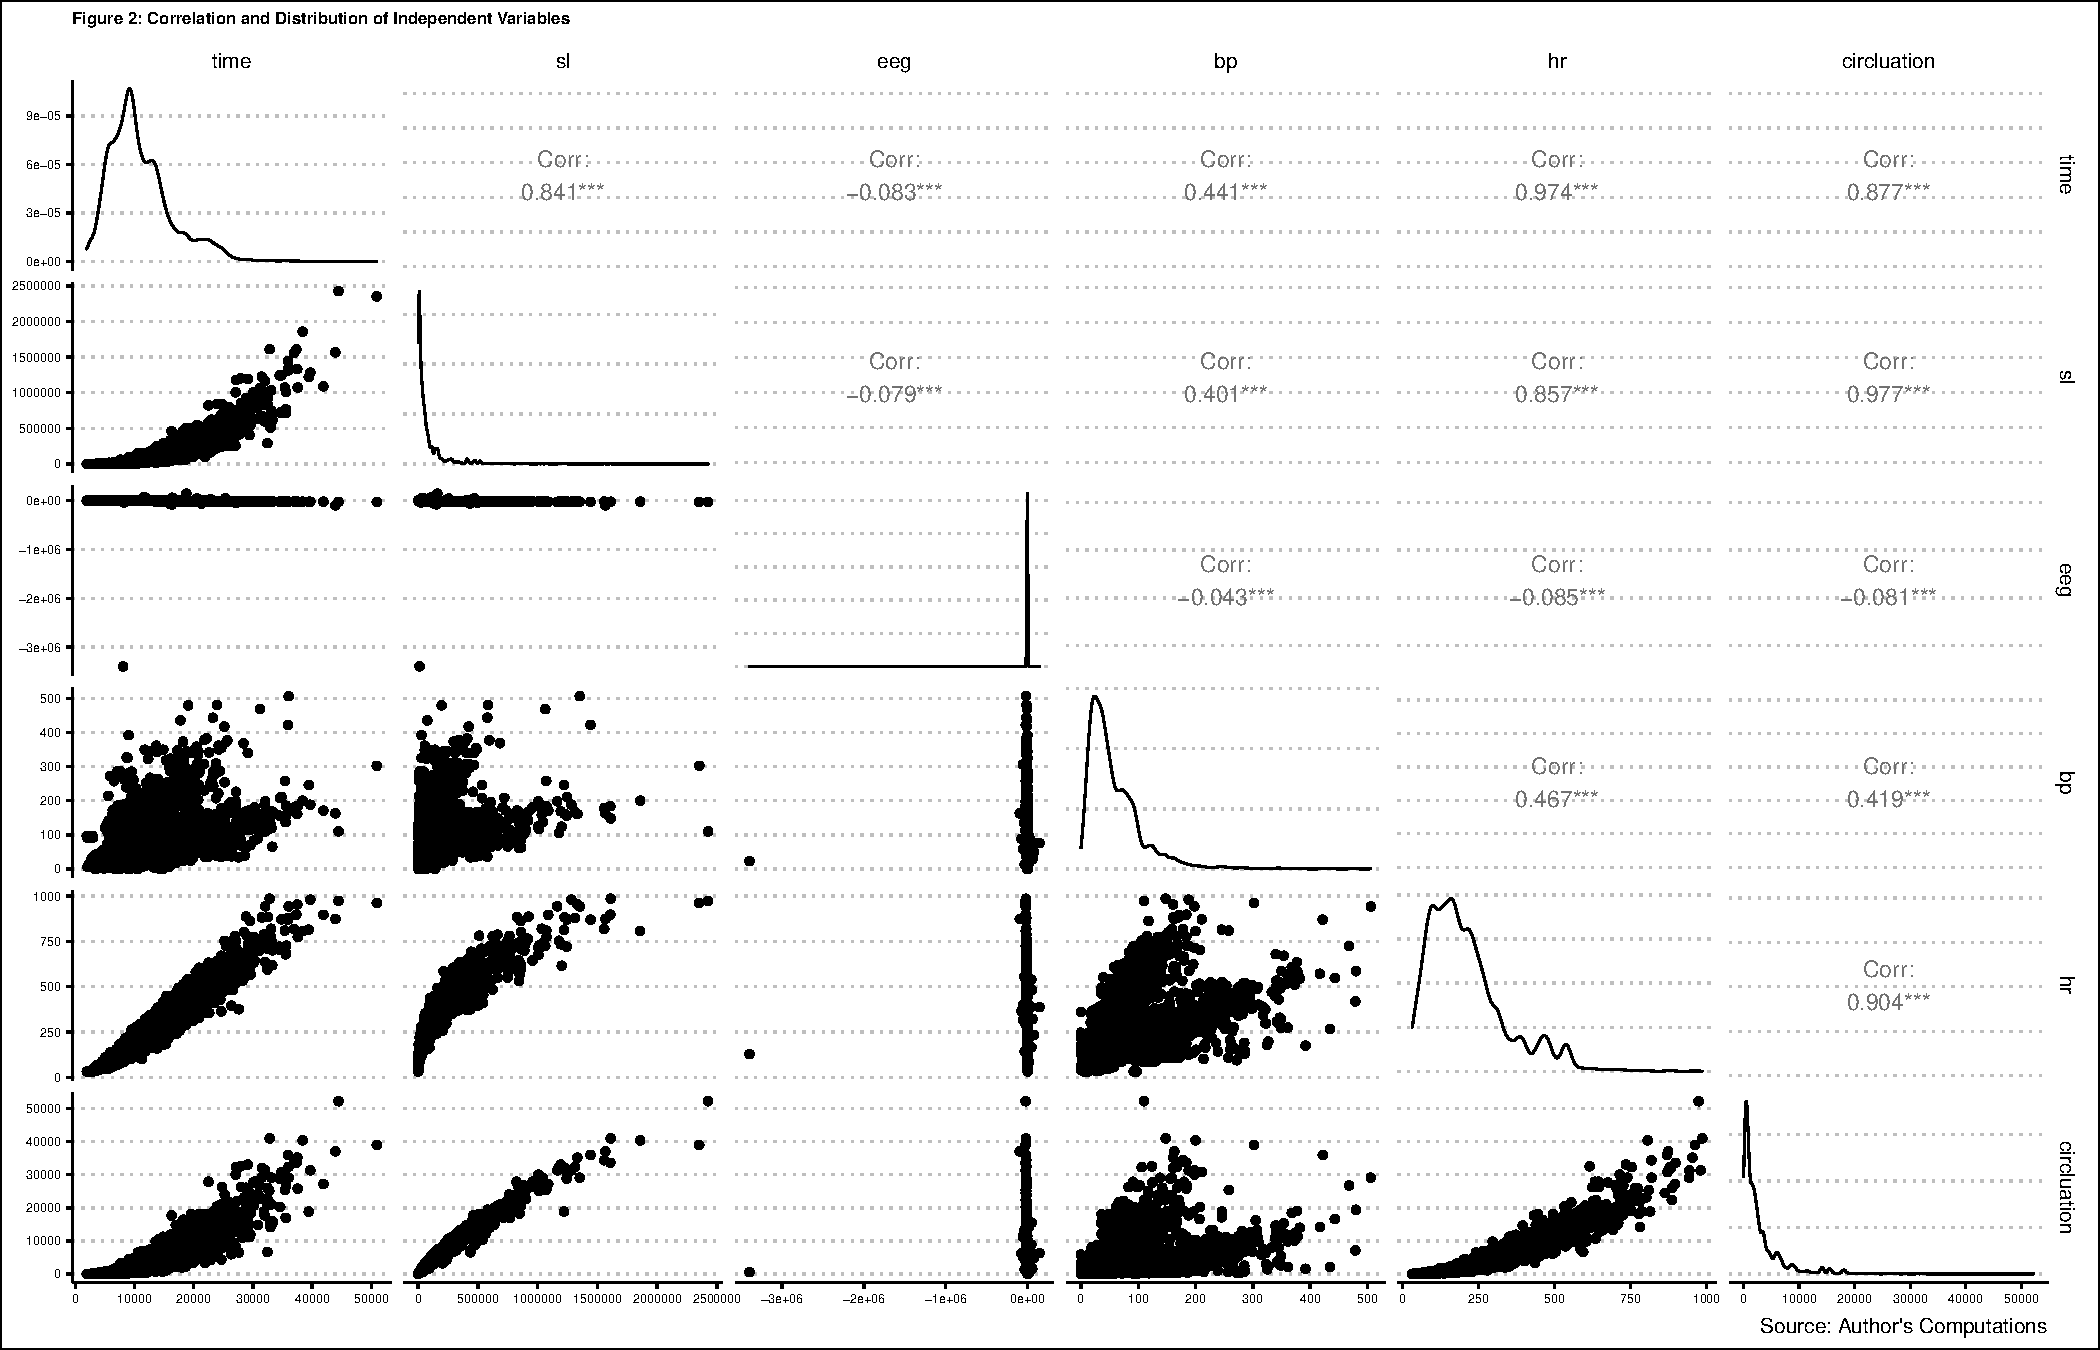
\includegraphics{karuitha_wits_bmi_files/figure-latex/unnamed-chunk-9-1.pdf}

\end{landscape}

I also visualize each of the principal components faceted by the
\texttt{Body\_Fat\_Level} defined above.

\begin{landscape}

\includegraphics{karuitha_wits_bmi_files/figure-latex/unnamed-chunk-10-1.pdf}

\end{landscape}

lastly, we examine the correlation between PC1, PC2 and PC3 and the
variables of BodyFat dataset. Table () shows that PC1 has very high
correlation with most of the variables. For instance, PC1 has a
correlation greater than 0.7 (absolute value) with 7 of the 11
independent variables. PC2 is not so strong but still has a correlation
above 0.6 (absolute) with 2 variables, while PC3 has a correlation
greater than 0.6 with one variable. In this case, it appears like PC1
and PC2 are adequate to capture most of the variability in the data.

\begin{tabular}{l|r|r|r}
\hline
  & PC1 & PC2 & PC3\\
\hline
density & -0.6907 & 0.5089 & -0.1076\\
\hline
age & 0.0611 & -0.6994 & -0.6774\\
\hline
weight & 0.9722 & 0.1027 & -0.0003\\
\hline
height & 0.2198 & 0.6965 & -0.4702\\
\hline
adiposity & 0.9220 & -0.2296 & 0.1318\\
\hline
thigh & 0.8920 & 0.1263 & 0.2964\\
\hline
abdomen & 0.9259 & -0.2718 & -0.0011\\
\hline
ankle & 0.6535 & 0.3575 & -0.1102\\
\hline
hip & 0.9493 & 0.0319 & 0.1551\\
\hline
wrist & 0.7483 & 0.1226 & -0.4507\\
\hline
knee & 0.8806 & 0.1548 & -0.0593\\
\hline
\end{tabular}

\hypertarget{regression-analysis}{%
\subsection{\texorpdfstring{\textbf{2.4 Regression
Analysis}}{2.4 Regression Analysis}}\label{regression-analysis}}

In this section, I start by doing a forward stepwise regression followed
by the required backward stepwise regression. Forward stepwise
regression starts with no independent variables in the model and
iteratively adds predictors that are the most significant. The process
stops when the improvement is no longer statistically significant. On
the contrary, the backward stepwise regression starts with all the
independent variables in the model and removes the least contributing
variables until all variables remaining are significant (Bruce, Bruce,
and Gedeck 2020)(James et al. 2013).

\hypertarget{forward-stepwise-regression}{%
\subsubsection{\texorpdfstring{\textbf{2.4.1 Forward Stepwise
Regression}}{2.4.1 Forward Stepwise Regression}}\label{forward-stepwise-regression}}

I include the forward stepwise selection method for purposes of
comparison. Note that the optimal model here includes all variables,
although only the density is significant. Overall, the model captures
97.74\% of the variation in body fat (see adjusted R squared in the
table below).

\begin{verbatim}
## Start:  AIC=88.26
## bodyfat ~ density + age + weight + height + adiposity + thigh + 
##     abdomen + ankle + hip + wrist + knee
\end{verbatim}

\begin{verbatim}
## 
## Call:
## lm(formula = bodyfat ~ density + age + weight + height + adiposity + 
##     thigh + abdomen + ankle + hip + wrist + knee, data = BodyFat4)
## 
## Residuals:
##    Min     1Q Median     3Q    Max 
## -7.787 -0.301 -0.075  0.175 14.245 
## 
## Coefficients:
##              Estimate Std. Error t value Pr(>|t|)    
## (Intercept)  4.20e+02   9.32e+00   45.11   <2e-16 ***
## density     -3.81e+02   7.36e+00  -51.78   <2e-16 ***
## age          9.34e-03   8.62e-03    1.08     0.28    
## weight       1.32e-02   1.27e-02    1.04     0.30    
## height      -1.94e-02   3.01e-02   -0.64     0.52    
## adiposity   -4.08e-02   7.37e-02   -0.55     0.58    
## thigh       -1.93e-02   3.76e-02   -0.51     0.61    
## abdomen      3.50e-02   2.82e-02    1.24     0.22    
## ankle       -7.04e-02   5.98e-02   -1.18     0.24    
## hip          1.18e-02   3.74e-02    0.32     0.75    
## wrist        2.45e-02   1.37e-01    0.18     0.86    
## knee        -3.06e-02   6.63e-02   -0.46     0.64    
## ---
## Signif. codes:  0 '***' 0.001 '**' 0.01 '*' 0.05 '.' 0.1 ' ' 1
## 
## Residual standard error: 1.16 on 240 degrees of freedom
## Multiple R-squared:  0.978,  Adjusted R-squared:  0.977 
## F-statistic:  990 on 11 and 240 DF,  p-value: <2e-16
\end{verbatim}

\hypertarget{backward-stepwise-regression}{%
\subsubsection{\texorpdfstring{\textbf{2.4.2 Backward Stepwise
Regression}}{2.4.2 Backward Stepwise Regression}}\label{backward-stepwise-regression}}

As noted, backward step selection begins with all the variables in the
model and iteratively removes the least contributive ones. The Akaike
Information Citerion (AIC) informs the selection of the best model, with
the optimal model being the one with the least AIC. The series of tables
below show the procedure (note the AIC value stated at the beginning of
each model). In the end, the model consisting of density, age, and
abdomen as independent variables has the least AIC (75.39). Note that
the model selected in this case is as follows ;

bodyfat = 0.041 - (0.038 * density) + (9.51 * age) + (0.048 * abdomen)

The AIC captures the extent to which the model fits the data without
being overly complex. Complexity refers to the number of parameters in
the model and fittingly, AIC is the difference between the number of
parameters in the model (k) and the maximum value of the likelihood
function of the model (L).

AIC = (2 * k ) - (2 * ln(L)), where ln stands for natural log.

The central idea of AIC is to balance between fitting the data and the
need not to overfit the dataset (Portet 2020).

The model is captured at the bottom of the series of tables. In the
model, only age is not significant at 10\% significance level. As
expected, the model explains 97.79\% of the variation in body fat - the
adjusted R-Squared - which is a high level of in sample sensitivity. The
adjusted R-Squared derives from the R-squared, a goodness-of-fit measure
for linear regression models that indicates the percentage of the
variance in the dependent variable that the independent variables
explain collectively (Frost 2019b). Like the AIC, the adjusted R-squared
penalizes the R-squared as the model gets more complex, that is, gets
more predictors.

In our body fat case, body fat is negatively related to body fat.
Specifically, for every one unit increase in density, body fat reduces
by 0.038 units (rounded to two decimal places). Abdomen relates
positively with body fat with a one unit rise in abdomen associated with
0.048 units rise in body fat. Although not significant at 10\%, age has
a positive relationship with body fat, with a one unit increase in age
associated with a 9.5 units rise in body fat, a relatively large amount.

Furthermore the model as a whole is highly significant going by the
F-test . The F-test of overall significance tests how well the linear
regression model better fits the data compared to a model that has no
independent variables or in other words where the coefficients of the
independent variables are all zero. In out case the F-test is highly
significant meaning that the model better explains the model better than
a model with no predictors. If our model fits the data just as well as a
model with no predictors, then the F\_statistic should be close to one.
In this case it is 3703.

\begin{verbatim}
## Start:  AIC=88.26
## bodyfat ~ density + age + weight + height + adiposity + thigh + 
##     abdomen + ankle + hip + wrist + knee
## 
##             Df Sum of Sq  RSS AIC
## - wrist      1         0  325  86
## - hip        1         0  325  86
## - knee       1         0  325  86
## - thigh      1         0  326  87
## - adiposity  1         0  326  87
## - height     1         1  326  87
## - weight     1         1  327  87
## - age        1         2  327  87
## - ankle      1         2  327  88
## - abdomen    1         2  327  88
## <none>                    325  88
## - density    1      3633 3958 716
## 
## Step:  AIC=86.29
## bodyfat ~ density + age + weight + height + adiposity + thigh + 
##     abdomen + ankle + hip + knee
## 
##             Df Sum of Sq  RSS AIC
## - hip        1         0  325  84
## - knee       1         0  326  85
## - thigh      1         0  326  85
## - adiposity  1         0  326  85
## - height     1         1  326  85
## - weight     1         2  327  86
## - ankle      1         2  327  86
## - abdomen    1         2  327  86
## - age        1         2  327  86
## <none>                    325  86
## - density    1      3792 4117 724
## 
## Step:  AIC=84.38
## bodyfat ~ density + age + weight + height + adiposity + thigh + 
##     abdomen + ankle + knee
## 
##             Df Sum of Sq  RSS AIC
## - knee       1         0  326  83
## - thigh      1         0  326  83
## - adiposity  1         0  326  83
## - height     1         1  326  83
## - ankle      1         2  327  84
## - age        1         2  327  84
## - abdomen    1         2  328  84
## - weight     1         2  328  84
## <none>                    325  84
## - density    1      3823 4149 724
## 
## Step:  AIC=82.57
## bodyfat ~ density + age + weight + height + adiposity + thigh + 
##     abdomen + ankle
## 
##             Df Sum of Sq  RSS AIC
## - adiposity  1         0  326  81
## - thigh      1         1  326  81
## - height     1         1  326  81
## - age        1         2  327  82
## - weight     1         2  328  82
## - ankle      1         2  328  82
## - abdomen    1         2  328  82
## <none>                    326  83
## - density    1      3823 4149 722
## 
## Step:  AIC=80.78
## bodyfat ~ density + age + weight + height + thigh + abdomen + 
##     ankle
## 
##           Df Sum of Sq  RSS AIC
## - height   1         0  326  79
## - thigh    1         1  326  79
## - age      1         2  328  80
## - weight   1         2  328  80
## - abdomen  1         2  328  80
## - ankle    1         2  328  81
## <none>                  326  81
## - density  1      3823 4149 720
## 
## Step:  AIC=79.05
## bodyfat ~ density + age + weight + thigh + abdomen + ankle
## 
##           Df Sum of Sq  RSS AIC
## - thigh    1         0  327  77
## - weight   1         2  328  78
## - age      1         2  328  79
## - ankle    1         2  329  79
## <none>                  326  79
## - abdomen  1         3  329  79
## - density  1      3834 4160 719
## 
## Step:  AIC=77.36
## bodyfat ~ density + age + weight + abdomen + ankle
## 
##           Df Sum of Sq  RSS AIC
## - weight   1         1  328  76
## - ankle    1         2  329  77
## - abdomen  1         3  329  77
## <none>                  327  77
## - age      1         3  330  78
## - density  1      3911 4237 721
## 
## Step:  AIC=76.29
## bodyfat ~ density + age + abdomen + ankle
## 
##           Df Sum of Sq  RSS AIC
## - ankle    1         1  329  75
## - age      1         2  330  76
## <none>                  328  76
## - abdomen  1        25  352  93
## - density  1      4475 4803 751
## 
## Step:  AIC=75.39
## bodyfat ~ density + age + abdomen
## 
##           Df Sum of Sq  RSS AIC
## <none>                  329  75
## - age      1         3  333  76
## - abdomen  1        24  354  91
## - density  1      4601 4930 755
\end{verbatim}

\begin{verbatim}
## 
## Call:
## lm(formula = bodyfat ~ density + age + abdomen, data = BodyFat4)
## 
## Residuals:
##    Min     1Q Median     3Q    Max 
## -7.716 -0.308 -0.078  0.207 14.460 
## 
## Coefficients:
##              Estimate Std. Error t value Pr(>|t|)    
## (Intercept)  4.14e+02   7.68e+00   53.91  < 2e-16 ***
## density     -3.79e+02   6.44e+00  -58.87  < 2e-16 ***
## age          9.51e-03   6.01e-03    1.58     0.11    
## abdomen      4.80e-02   1.12e-02    4.28  2.7e-05 ***
## ---
## Signif. codes:  0 '***' 0.001 '**' 0.01 '*' 0.05 '.' 0.1 ' ' 1
## 
## Residual standard error: 1.15 on 248 degrees of freedom
## Multiple R-squared:  0.978,  Adjusted R-squared:  0.978 
## F-statistic: 3.7e+03 on 3 and 248 DF,  p-value: <2e-16
\end{verbatim}

\hypertarget{checking-the-regression-assumptions}{%
\subsubsection{\texorpdfstring{\textbf{2.4.3 Checking the Regression
Assumptions}}{2.4.3 Checking the Regression Assumptions}}\label{checking-the-regression-assumptions}}

In this section, I work with the regression model selected in section 5
above- which uses density, age and abdomen as independent variables. The
regression has five key assumptions:

\begin{itemize}
\item
  \emph{Linear relationship}: here, the assumption is that the
  relationship between the dependent and the independent variables is
  linear. a visual inspection of the figure 3.1 (see section 3) shows
  that with the exception of age, the relationship between body fat and
  the independent variables is approximately linear. Furthermore in the
  figure below, the plot titled residuals versus fitted also largely
  coloborates the linear relationship between dependent and independent
  variables.
\item
  \emph{Multivariate normality}: The presumption here is that all
  variables are multivariate normal. I check this assumption with the
  normal QQ-plot below. In this case, the plotted residuals versus
  theoretical quantiles show that the assumption is reasonably met as
  they lie on approximately the straight line.
\item
  \emph{No or little multicollinearity}. There appears to be a violation
  of this assumption as density and abdomen have a high negative
  correlation coefficient.
\end{itemize}

\begin{tabular}{l|r|r}
\hline
  & age & abdomen\\
\hline
density & -0.2776 & -0.799\\
\hline
\end{tabular}

In this case, \textbf{I remove the least contributive variable},
abdomen, and rerun the model.

\begin{verbatim}
## 
## Call:
## lm(formula = bodyfat ~ density + age, data = BodyFat4)
## 
## Residuals:
##    Min     1Q Median     3Q    Max 
## -8.103 -0.215 -0.094  0.051 15.718 
## 
## Coefficients:
##              Estimate Std. Error t value Pr(>|t|)    
## (Intercept)  4.41e+02   4.43e+00   99.66   <2e-16 ***
## density     -4.01e+02   4.11e+00  -97.38   <2e-16 ***
## age          9.89e-03   6.21e-03    1.59     0.11    
## ---
## Signif. codes:  0 '***' 0.001 '**' 0.01 '*' 0.05 '.' 0.1 ' ' 1
## 
## Residual standard error: 1.19 on 249 degrees of freedom
## Multiple R-squared:  0.977,  Adjusted R-squared:  0.976 
## F-statistic: 5.19e+03 on 2 and 249 DF,  p-value: <2e-16
\end{verbatim}

Note that this simplified model consisting of density and age (to the
exclusion of abdomen) captures most of the information. The adjusted
R-squared is 97.64\% compared to 97.79\% of the previous model that
included abdomen. Age remains insignificant in both cases (10\%
significant level).

\begin{itemize}
\item
  \emph{No auto-correlation}: The data has not time element so we do not
  evaluate this assumption.
\item
  \emph{Homoscedasticity}: In the figure below, the graph titled ``scale
  location'' provides a useful assessment of how residuals are evenly
  spread across the predictors. In this case, the roughly horizontal fit
  line indicates that the residuals are homoscedastic.
\end{itemize}

Another important issue arising here is that of some influential
observations (outliers) the graph titled residuals versus leverage
shows. In this case, there is an influential observation that may affect
our inferences.

\includegraphics{karuitha_wits_bmi_files/figure-latex/unnamed-chunk-16-1.pdf}
\includegraphics{karuitha_wits_bmi_files/figure-latex/unnamed-chunk-16-2.pdf}
\includegraphics{karuitha_wits_bmi_files/figure-latex/unnamed-chunk-16-3.pdf}
\includegraphics{karuitha_wits_bmi_files/figure-latex/unnamed-chunk-16-4.pdf}

\hypertarget{hypothesis-tests-for-the-parameters}{%
\subsubsection{\texorpdfstring{\textbf{2.4.4 Hypothesis Tests for the
Parameters}}{2.4.4 Hypothesis Tests for the Parameters}}\label{hypothesis-tests-for-the-parameters}}

The final model selected is as folows.

bodyfat = a + b1(density) + bn(factor(age\_group)) + error

where a is a constant and b1 and bn are respective coefficients. Note
that bn coefficients will be for each of the categories representing age
less the reference category (age 22 years). I test the foloowing
hypothesis.

\begin{itemize}
\item
  For density: NULL: b1 = 0, versus alternative b1 != 0 P-value is close
  to zero meaning that there is very little probability that the null
  hypothesis is true. having failed to accept the null hypothesis we go
  with the alternative hypothesis.
\item
  For age: NULL: bn = 0, versus alternative bn != 0 Likewise, for each
  age category, the probabilities are quite large (\textgreater{} 10\%).
  Hence in this case we accept the null hypothesis that age is not a
  significant determinant of body fat.
\item
  The overall model fit: The F-test As noted the F-test evaluates
  whether our model does better than a model with no predictors. As a
  ratio, if our model does just as well as that with no predictors, the
  F-ratio would be close to one.
\end{itemize}

NULL: b1 = bn = 0 Alternative: b1 != 0 and bn != 0

The F-statistic is 274.6 and the p-value is close to zero, meaning that
we cannot accept the null hypothesis and hence go with the alternative
hypothesis that our model is better than a model with no predictors.

The associated degree of freedom in our case are 51 and 200.

\hypertarget{the-final-model--making-age-a-categorical-variable}{%
\subsubsection{\texorpdfstring{\textbf{2.4.5 The Final Model- Making age
a Categorical
Variable}}{2.4.5 The Final Model- Making age a Categorical Variable}}\label{the-final-model--making-age-a-categorical-variable}}

One of the steps in selecting the model is dropping one of the
independent variable, abdomen, that is highly related to another
independent variable, density. A final procedure is to convert age to a
categorical variable. Technically, age is a continuous variable measured
on a ratio scale as we have a true zero for age. Age maybe considered
discrete because of the way it is measured. Specifically, age suffers
from the ``discretization'' problem where people do not record their
exact age, preferring instead to round up to the nearest year. In the
case of body fat, the effect of age on body fat may not be apparent at
exact age points but on a range of age groups. We could say, for
instance that people between ages 20-30 years have lower body fat than
those between 30 - 40 years. In this case, I translate the age to a
categorical variable and re-run the analysis. The analysis shows that
encoding age as a categorical variable does improve the model to one
with an adjusted R-squared of 97.64\%. Thus the model with density and
age explains 97.64\% of the variation in body fat.

I encode the age variable into the following categories and rerun the
regression model; 20 - 29 year 30 - 39 years 40 - 49 years 50 - 59 years
Over 60 years

I call the new variable age\_group.

\begin{verbatim}
## 
## Call:
## lm(formula = bodyfat ~ density + factor(age_group), data = BodyFat4)
## 
## Residuals:
##    Min     1Q Median     3Q    Max 
## -7.843 -0.221 -0.087  0.099 15.541 
## 
## Coefficients:
##                           Estimate Std. Error t value Pr(>|t|)    
## (Intercept)               442.1962     4.4629   99.08   <2e-16 ***
## density                  -401.0903     4.1804  -95.95   <2e-16 ***
## factor(age_group)30-39     -0.1900     0.2772   -0.69     0.49    
## factor(age_group)40-49      0.0987     0.2392    0.41     0.68    
## factor(age_group)50-59      0.4014     0.2663    1.51     0.13    
## factor(age_group)Over 60    0.2832     0.2959    0.96     0.34    
## ---
## Signif. codes:  0 '***' 0.001 '**' 0.01 '*' 0.05 '.' 0.1 ' ' 1
## 
## Residual standard error: 1.19 on 246 degrees of freedom
## Multiple R-squared:  0.977,  Adjusted R-squared:  0.976 
## F-statistic: 2.08e+03 on 5 and 246 DF,  p-value: <2e-16
\end{verbatim}

\hypertarget{interpreting-the-results}{%
\subsubsection{\texorpdfstring{\textbf{2.4.6 Interpreting the
Results}}{2.4.6 Interpreting the Results}}\label{interpreting-the-results}}

For the final model that consists of density and age (coded as factors)
the interpretation of the results is as follows.

Density: Density is a significant determinant of body fat. Age also
appears to be an important factor but is not significant. Although
abdomen is significant, density alone appears to subsume the effects of
abdomen.

\hypertarget{limitations}{%
\section{\texorpdfstring{\textbf{Limitations}}{Limitations}}\label{limitations}}

Disusss limitations here - for instance is the dataset too small? Can we
generalize this to the whole world given genetic differences? You are
the expert in the area so you should get the limitations in the books.

\hypertarget{conclusion}{%
\section{\texorpdfstring{\textbf{3
Conclusion}}{3 Conclusion}}\label{conclusion}}

Overall it appears that the best predictors of body fat are density and
age. However, only density is significant, with a 1 unit rise in density
associating with a 401 unit decrease in body fat.

\hypertarget{references}{%
\section*{\texorpdfstring{\textbf{References}}{References}}\label{references}}
\addcontentsline{toc}{section}{\textbf{References}}

\hypertarget{refs}{}
\begin{CSLReferences}{1}{0}
\leavevmode\vadjust pre{\hypertarget{ref-bruce2020practical}{}}%
Bruce, Peter, Andrew Bruce, and Peter Gedeck. 2020. \emph{Practical
Statistics for Data Scientists: 50+ Essential Concepts Using r and
Python}. O'Reilly Media.

\leavevmode\vadjust pre{\hypertarget{ref-frost2019introduction}{}}%
Frost, J. 2019a. {``Introduction to Statistics: An Intuitive Guide.''}
\emph{Statistics by Jim Publishing}, 196--204.

\leavevmode\vadjust pre{\hypertarget{ref-frost2019regression}{}}%
---------. 2019b. {``Regression Analysis: An Intuitive Guide.''} E-book.

\leavevmode\vadjust pre{\hypertarget{ref-james2013introduction}{}}%
James, Gareth, Daniela Witten, Trevor Hastie, and Robert Tibshirani.
2013. \emph{An Introduction to Statistical Learning}. Vol. 112.
Springer.

\leavevmode\vadjust pre{\hypertarget{ref-jolliffe2016principal}{}}%
Jolliffe, Ian T, and Jorge Cadima. 2016. {``Principal Component
Analysis: A Review and Recent Developments.''} \emph{Philosophical
Transactions of the Royal Society A: Mathematical, Physical and
Engineering Sciences} 374 (2065): 20150202.

\leavevmode\vadjust pre{\hypertarget{ref-portet2020primer}{}}%
Portet, Stéphanie. 2020. {``A Primer on Model Selection Using the Akaike
Information Criterion.''} \emph{Infectious Disease Modelling} 5:
111--28.

\leavevmode\vadjust pre{\hypertarget{ref-7835187}{}}%
Zhu, J., Z. Ge, and Z. Song. 2017. {``Distributed Parallel PCA for
Modeling and Monitoring of Large-Scale Plant-Wide Processes with Big
Data.''} \emph{IEEE Transactions on Industrial Informatics} 13 (4):
1877--85.

\end{CSLReferences}

\end{document}
